\documentclass[a4paper]{article}
\usepackage[titletoc]{appendix}
% http://faculty.uoit.ca/bohun/latex/margins.html
\usepackage[a4paper,left=2.5cm,top=3.2cm,right=2.5cm,bottom=2.54cm,nohead,nofoot]{geometry}
\usepackage{fancyhdr}
\usepackage{url}
\usepackage{amsmath,amssymb,amsthm}
\usepackage{color,graphicx,subfigure,enumerate,epsfig,epstopdf}
\usepackage{listings}

\newcommand{\etal}{\emph{et al.} }

\title{A Framework for Personalized Apparel Recommendation}

\author{
Xiao Jia\\
        \small Shanghai Jiao Tong University\\
        \small \texttt{xjia@cs.sjtu.edu.cn}\\
\and
Junjia He\\
        \small Shanghai Jiao Tong University\\
        \small \texttt{hejunjia1911@gmail.com}\\
\and
Wei Li\\
        \small Shanghai Jiao Tong University\\
        \small \texttt{liwei606@gmail.com}\\
}

\date{}

\begin{document}
\maketitle

\begin{abstract}
In E-commerce systems, picking an item is time-consuming for individuals, which demands recommender systems with higher efficiency and accuracy, as well as support for more personalized recommendation. We propose a novel idea and framework for personalized apparel recommendation which combines both item images and textual labels by using sparse coding and support vector machine (SVM). Extensive discussions and preliminary experiment results show the practicality and validity of our framework.
\end{abstract}

\tableofcontents

\newpage

\section{Introduction}\label{sec:intro}

% P1: Motivation. 
% - What is the problem area you are working in and why is it important? 
% - Why is the problem of interest and importance to the larger community?
Recommender systems have become a hot research area in recent years and 
  many innovative approaches have been proposed both scientifically and commercially. 
Many recommender systems deal with books and daily commodities; 
  they need to be more efficient and accurate, and cover more fields.
Online trading is an overwhelming trend and E-commerce is a promising field. 
For many businesses, online opinion has turned into a kind of virtual currency 
  that can make or break a product in the marketplace \cite{Wright09}. 
There are so many items (products) in E-commerce systems that 
  picking an item is time-consuming for individuals.
Therefore recommender systems are key to the success of such E-commerce systems, 
  and shortening the time for an individual means improving the 
  throughput of the E-commerce system, thus contributing more transactions.

% P2: What is the specific problem considered in this paper? 
The soaring E-commerce industry demands recommender systems 
  with higher efficiency and accuracy, as well as support for more 
  personalized recommendation.
Personalized recommendation can be achieved by using data mining techniques on 
  massive amount of user profiles and behaviors (so-called collaboration) 
  regardless of the features of recommended items themselves. 
However, this kind of personalized recommendation is not applicable to 
  personalized apparel recommendation where the choices of people with similar interests 
  are sensitive to apparel particulars and may differ in case of only tiny differences. 
In this case, it is essential to capture as many features as possible 
  which are associated with both the clothes themselves and the user's preference 
  so that the personalized recommendation can be achieved in better performance. 

% P3: Summarize what are the main contributions of your paper.
% - What is the general approach taken? 
% - Why are the specific results significant?
In this paper, we propose a novel idea and framework for personalized apparel recommendation
  which combines both item images and textual labels by using sparse coding and 
  support vector machine (SVM). 
Sparse coding provides a class of algorithms for finding succinct representations of stimuli; 
  given only unlabeled input data, it learns basis functions that capture higher-level features 
  in the data \cite{Lee07}.
SVM is a widely used machine learning method for classification and regression analysis,
  based on the principle of structural risk minimization, which performs well when applied to 
  data outside the training set \cite{El02}.

% P4: What are the differences in what you are doing, and what others have done?
Given the images, the textual descriptions and the user ratings of the garments,
  our framework is capable of personalized recommendation according to various metrics
  such as style and diversity.
The novelty of our approach also comes from the fact that
  we try to not only employ a reasonable method to utilize 
  image information but also combine the image and text information together.
To the best of our knowledge, personalized apparel recommendation has not been 
  studied before in the context of E-commerce systems and the combination of 
  image feature extraction and machine learning.

% P5  
The remainder of this paper is structured as follows. 
Section \ref{sec:overview} presents an overview of our framework. In Section \ref{sec:challenge} several technical challenges in personalized apparel recommendation are discussed.
Section \ref{sec:approach} presents our approach for the novel framework for personalized apparel recommendation.
Section \ref{sec:eval} shows some preliminary experiment results under our framework.
Section \ref{sec:conclusion} concludes this paper and discusses some future work.
Section \ref{sec:related} discusses some of the related work.




\section{Overview}\label{sec:overview}

\begin{figure}
  \centering
  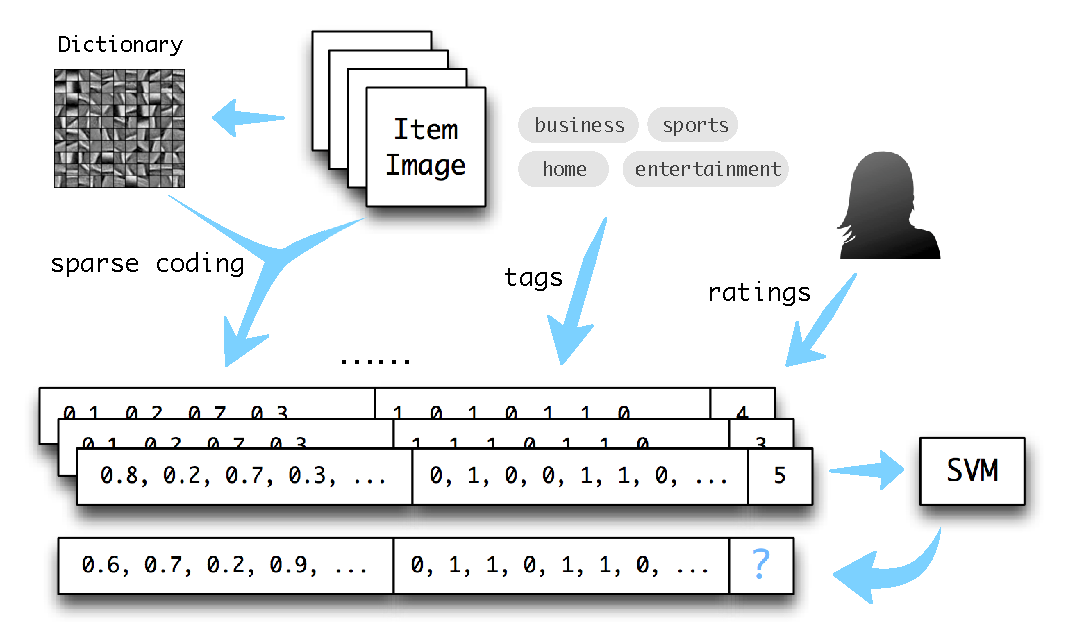
\includegraphics[width=0.9\textwidth]{framework}
  \caption{Framework Overview}
  \label{fig:overview}
\end{figure}

Our framework learned the features of clothing from both the textual labels and the images of clothes on the E-commerce websites. The input of our framework is the user preference which can be modeled from some of the user action records, including browsing time, favorite items, clicking history and ratings, etc. The output is the recommended clothes ranked by the possibility that the user would be interested in it. This framework has three major steps: learning clothing features,
modeling user preferences, and recommending by rating. Figure \ref{fig:overview} depicts the overall process of personalized recommendation in our framework.

\subsection{Learn clothing features}
There are two features we can leverage to model a garment item. One is textual labels such as cotton for material, sports for style and XL for size, etc. The other is several affiliated images depicting each garment. The information of textual labels and images would be represented as textual vectors and image vectors respectively. The representation of textual labels is quite straightforward as we can extract all the possible adjectives like slim, loose, lady and cute in the textual
labels. Each adjective represent a feature of the apparel in textual level. If the apparel item contains that feature in its textual label, we can mark 1 in the corresponding place in the textual vector. If not, mark 0. The image processing is more complicated than textual processing to learn the representations. We get the image vector from a base matrix which also serves as a dictionary. The technique details will be discussed in Section \ref{sec:approach}. After both the textual labels
and the images being represented as vectors, the two vectors will be combined together by weight as the final representation for each apparel item.

\subsection{Model user preference}
In our framework, each apparel item is linked with a preference model for a specific user, and the model would be applied to map the clothing set to the preference set of that user. For different users, the mapping from the clothing set to the corresponding preference set may vary significantly. Many actions can be tracked in the E-commerce systems to model the user preference such as scanning time, favorite collection, purchase records and even clicks, etc. These features can be modeled
as a rating with an approriate range, 1 to 5 for instance. Here we choose the rating to represent the user preference is reasonable since the model of user preference has a direct connection with the way we do recommendation. If we model the user preference with ratings then we can recommend by the predicted ratings of each garment evaluated by machine learning technology. Quantify the user preference is an accurate and easy way to do the recommendation. 

\subsection{Recommend by rating}
The last step of our framework is to recommend clothes in which the user has high possibility to invest. The ranking strategy of the recommendation is based on the value of possibility provided by the machine learning technology which takes both the vectors of apparel item and the corresponding ratings of user preference as the input set. In this step, the major technique we've leveraged is support vector machine (SVM) which can solve this kind of problem correctly and efficiently. More details can been seen in Section \ref{sec:approach}.\\
\\
In summary, there are three major contributions in this paper and our framework:
\begin{itemize}
	\item We propose a novel and more effective approach to build a framework for personalized apparel recommender systems which focus on the personality of different users and recommend with higher accuracy. We leverage all the possible information of each apparel item from both the textual labels and garment images. We combine the vectors of the two sources together by weight to represent the apparel item. The weight can be adaptive to different users as the emphasis on textual labels and images varied from person to person.
	\item We propose a novel way to leverage the different images affiliated to one apparel item. We treat these images as distinctive garment images with the same textual labels and ratings. For example, if an apparel item has ID 4 and contains 3 images I1 I2 I3 to dipict this garment along with a textual label T. If the corresponding preference of this garment has been known from a specific user and the rating is R. Then in our framework we treat these three images affiliated to the same
        apparel item as three distinctive items but with the same textual label T and the rating R. This process can enhance the efficiency of the item modeling and learning process.
	\item We have tried several algorithm that can be applied in our framework. As a consequence we managed to exclude the unsuitalbe ones and leverage the most efficient and suitable algorithms like HAC, K-SVD, SVM, etc.
\end{itemize}


\section{Technical Challenges}\label{sec:challenge}

In this section, several technical challenges in personalized apparel recommendation 
  are listed and discussed with respect to our framework. 

\subsection{How to Model an Item}
An \emph{item} means a garment along with several images and text labels.
For personalized apparel recommendation, one common way is to extract 
  the text labels (sizes, styles, colors, materials, etc.) and do recommendation 
  based on the statistics of and the relationships among these labels.
However, it ignores lots of information provided by the images of the garments.
As stated in Section \ref{sec:intro}, personalized apparel recommendation is 
  very much sensitive in that the choices of people with similar interests 
  may differ in case of only tiny differences. 
One of the novelties in our work is to model items by using the image features.
For image features, we strive to capture the most distinguishing or significant ones 
  in order to improve the sensitivity of our recommendation.

\subsection{How to Model User Preference}
In E-commerce systems, various actions can be captured and classified as user preferences,
  for example, viewing item page, checking details (mouse clicking), adding to cart, adding to favorites.
However, these kinds of actions are relatively easy to trigger and have less side effects.
So there tends to be many of these actions which may include noises and cause misleading recommendations.
In our framework, the users are required to judge a garment with scores based on personal preference,
  i.e. to give ratings manually.
Along with the scores, the users can also specify the confidence values of the rating. 
For those easy-to-trigger actions (or events), it is trivial to generate scores with appropriate 
  confidence values on behalf of the users.

\subsection{How to Recommend}
Given the item models and user preference models, the next problem to solve is how to recommend.
One possible way is to use a na\"ive Bayes classifier or similar probabilistic classifiers.
However, these kinds of classifiers require some extent of distribution independence which may not, 
  or relatively hard to, be satisfied under the setting of the item models and preference models. 
In our framework, the item models are required to be in the form of vectors, and an SVM classifier 
  is trained from user ratings of everybody and used as the preference model for each user.
Eventually there will be one SVM classifier for each user and the framework recommends according to
  the scores given by the classifier. 

\subsection{How to Recommend in an Online Context}
For any of the item modeling, the user preference modeling and the recommendation, 
  it should be done in an \emph{online} context because of the nature of E-commerce systems.
This means most of the batch-mode offline algorithms can not be applied in the framework.
Since this involves more fundamental aspects of image processing and machine learning, 
  instead of devising new techniques or reinventing the wheels, we examine and adopt several 
  suitable algorithms in our framework for further selection. 


\section{Our Approach}\label{sec:approach}

For images, at first they are preprocessed to gray-scale 
  pictures with minimum disturbance from the background 
  and the photo model, which is approached by morphological 
  manipulation using OpenCV. 
Then sparse coding is applied with respect to a learnt dictionary  
  to delineate pictures by feature vectors. 
Thus each image can be successfully represented and be ready for machine learning. 
It is also noted that if a garment contains several pictures, 
  it would be treated as several garments of the same text labels and scores.

As for text label processing, a certain number of keywords 
  could be picked to describe clothing characteristics like 
  \emph{long sleeve} in sleeve length, 
  \emph{leisure} in styles and 
  \emph{cotton} in fabrics. 
A vector in binary is used to record such features. 
Ultimately, they will be concatenated to another vector to represent clothing features. 
In addition, clustering is applied to detect the different text labels with the same meaning.

For every user, he or she will judge a garment based on personal 
  preference with scores from 1 to 5. 
All the choices for clothing are recorded for future recommendation. 
Then based on the certain user's previous choices, the potential 
  high-score garments can be predicted and thus being recommended.

Once we get the user's preferences (scores) on some garments, 
  the relationships between these garments and their scores on this
  particular user have been established, which are serving as a training set. 
Then we use SVM to estimate the scores of other garments, based on which, 
  we pick the highest ones to recommend. 
Note that this whole process is based on this particular user's preference.
There's also another optional way to recommend. 
The garments we recommend will have a high possibility of user's preference, 
  which is derived from the relationship between the preference models of different users.

Formally, suppose there are $K$ keywords in total, then every item $I$ has an associated 
  $K$-dimensional vector $T(I)$ where each dimension is either 0 or 1 which indicates the 
  existence of the corresponding keyword in the text labels of item $I$.
For an item $I$ and a user $U$, let $s(U,I)$ denote the score of $I$ given by $U$. 
Let $M(I)$ be the collection of all the images of $I$, $D$ be the learnt dictionary, and
  $C(M,D)$ be the sparse coding of $M$ using $D$.
Then the training set can be represented as $$ \{ [C(M^*,D), T(I), s(U,I)] : M^* \in M(I) \} .$$


\section{Evaluation}\label{sec:eval}
The proposed framework is temporarily evaluated in terms of its ability to model users' preferences solely based on text labels of garments regardless of the photos. The following subsections would separately describe our evaluation approaches and results.

\subsection{Experiment Settings}
At first we acquired the garment information from Taobao where one set of garment consists several pictures and a text label describing the garment. By this way we have got 1772 garments in total as our raw data. The next step is to convert the chromatic pictures into scalable gray-scale pictures by OpenCV. After this step the preprocessing is done. 
 
The next thing we need is to acquire the users' preferences, and fortunately we successfully invited 24 volunteers to assess the garments and rate them. Meanwhile we set up a website and record every volunteer's scoring, and as a consequent we got approximately 60 ratings per volunteer summing up to 1553 ratings in total.

When considering the text labels, we manually chose 322 keywords as text features and Figure \ref{fig:freq} shows the frequency of each feature label. In the $Y$ axis are the frequencies, i.e. how many times a feature label appears in the set of text descriptions of rated garments, while the $X$ axis are the IDs of each feature label.

Temporarily we only focused on text label part, and ignore the pictures. And as for the selection of learning machines, we finally chose LIBSVM \cite{CC01a} as the tool to perform SVM learning.

\begin{figure}
  \centering
  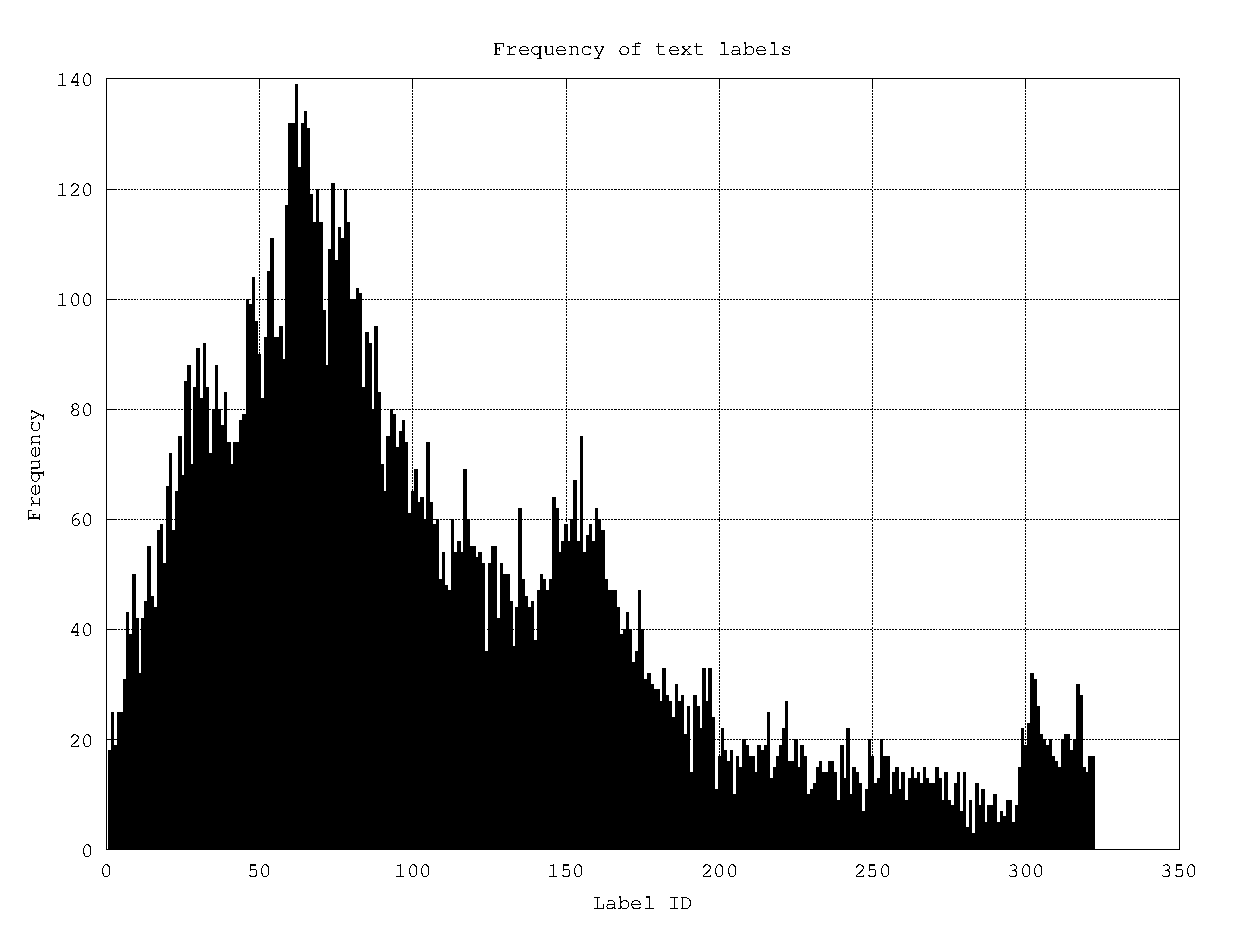
\includegraphics[width=0.9\textwidth]{frequency}
  \caption{Text label frequency}
  \label{fig:freq}
\end{figure}

\subsection{Website}

The section describes the website we set up for collecting user preferences.

Figure \ref{fig:website} shows the screenshots of the website.
Figure \ref{fig:website1} is a synthesized screenshot of both \emph{user rating} (top right) and \emph{product recommending} (middle right) user interface. The top left part shows the images of the product. When the user moves the mouse pointer over the image, a larger image will be shown in the top right part, as shown in \ref{fig:website2}. The bottom part of the page shows the textual descriptions of the product.

\begin{figure}[htb]
  \centering
  \subfigure[Synthesized screenshot of both \emph{user rating} and \emph{product recommending} user interface]{
    \label{fig:website1}
    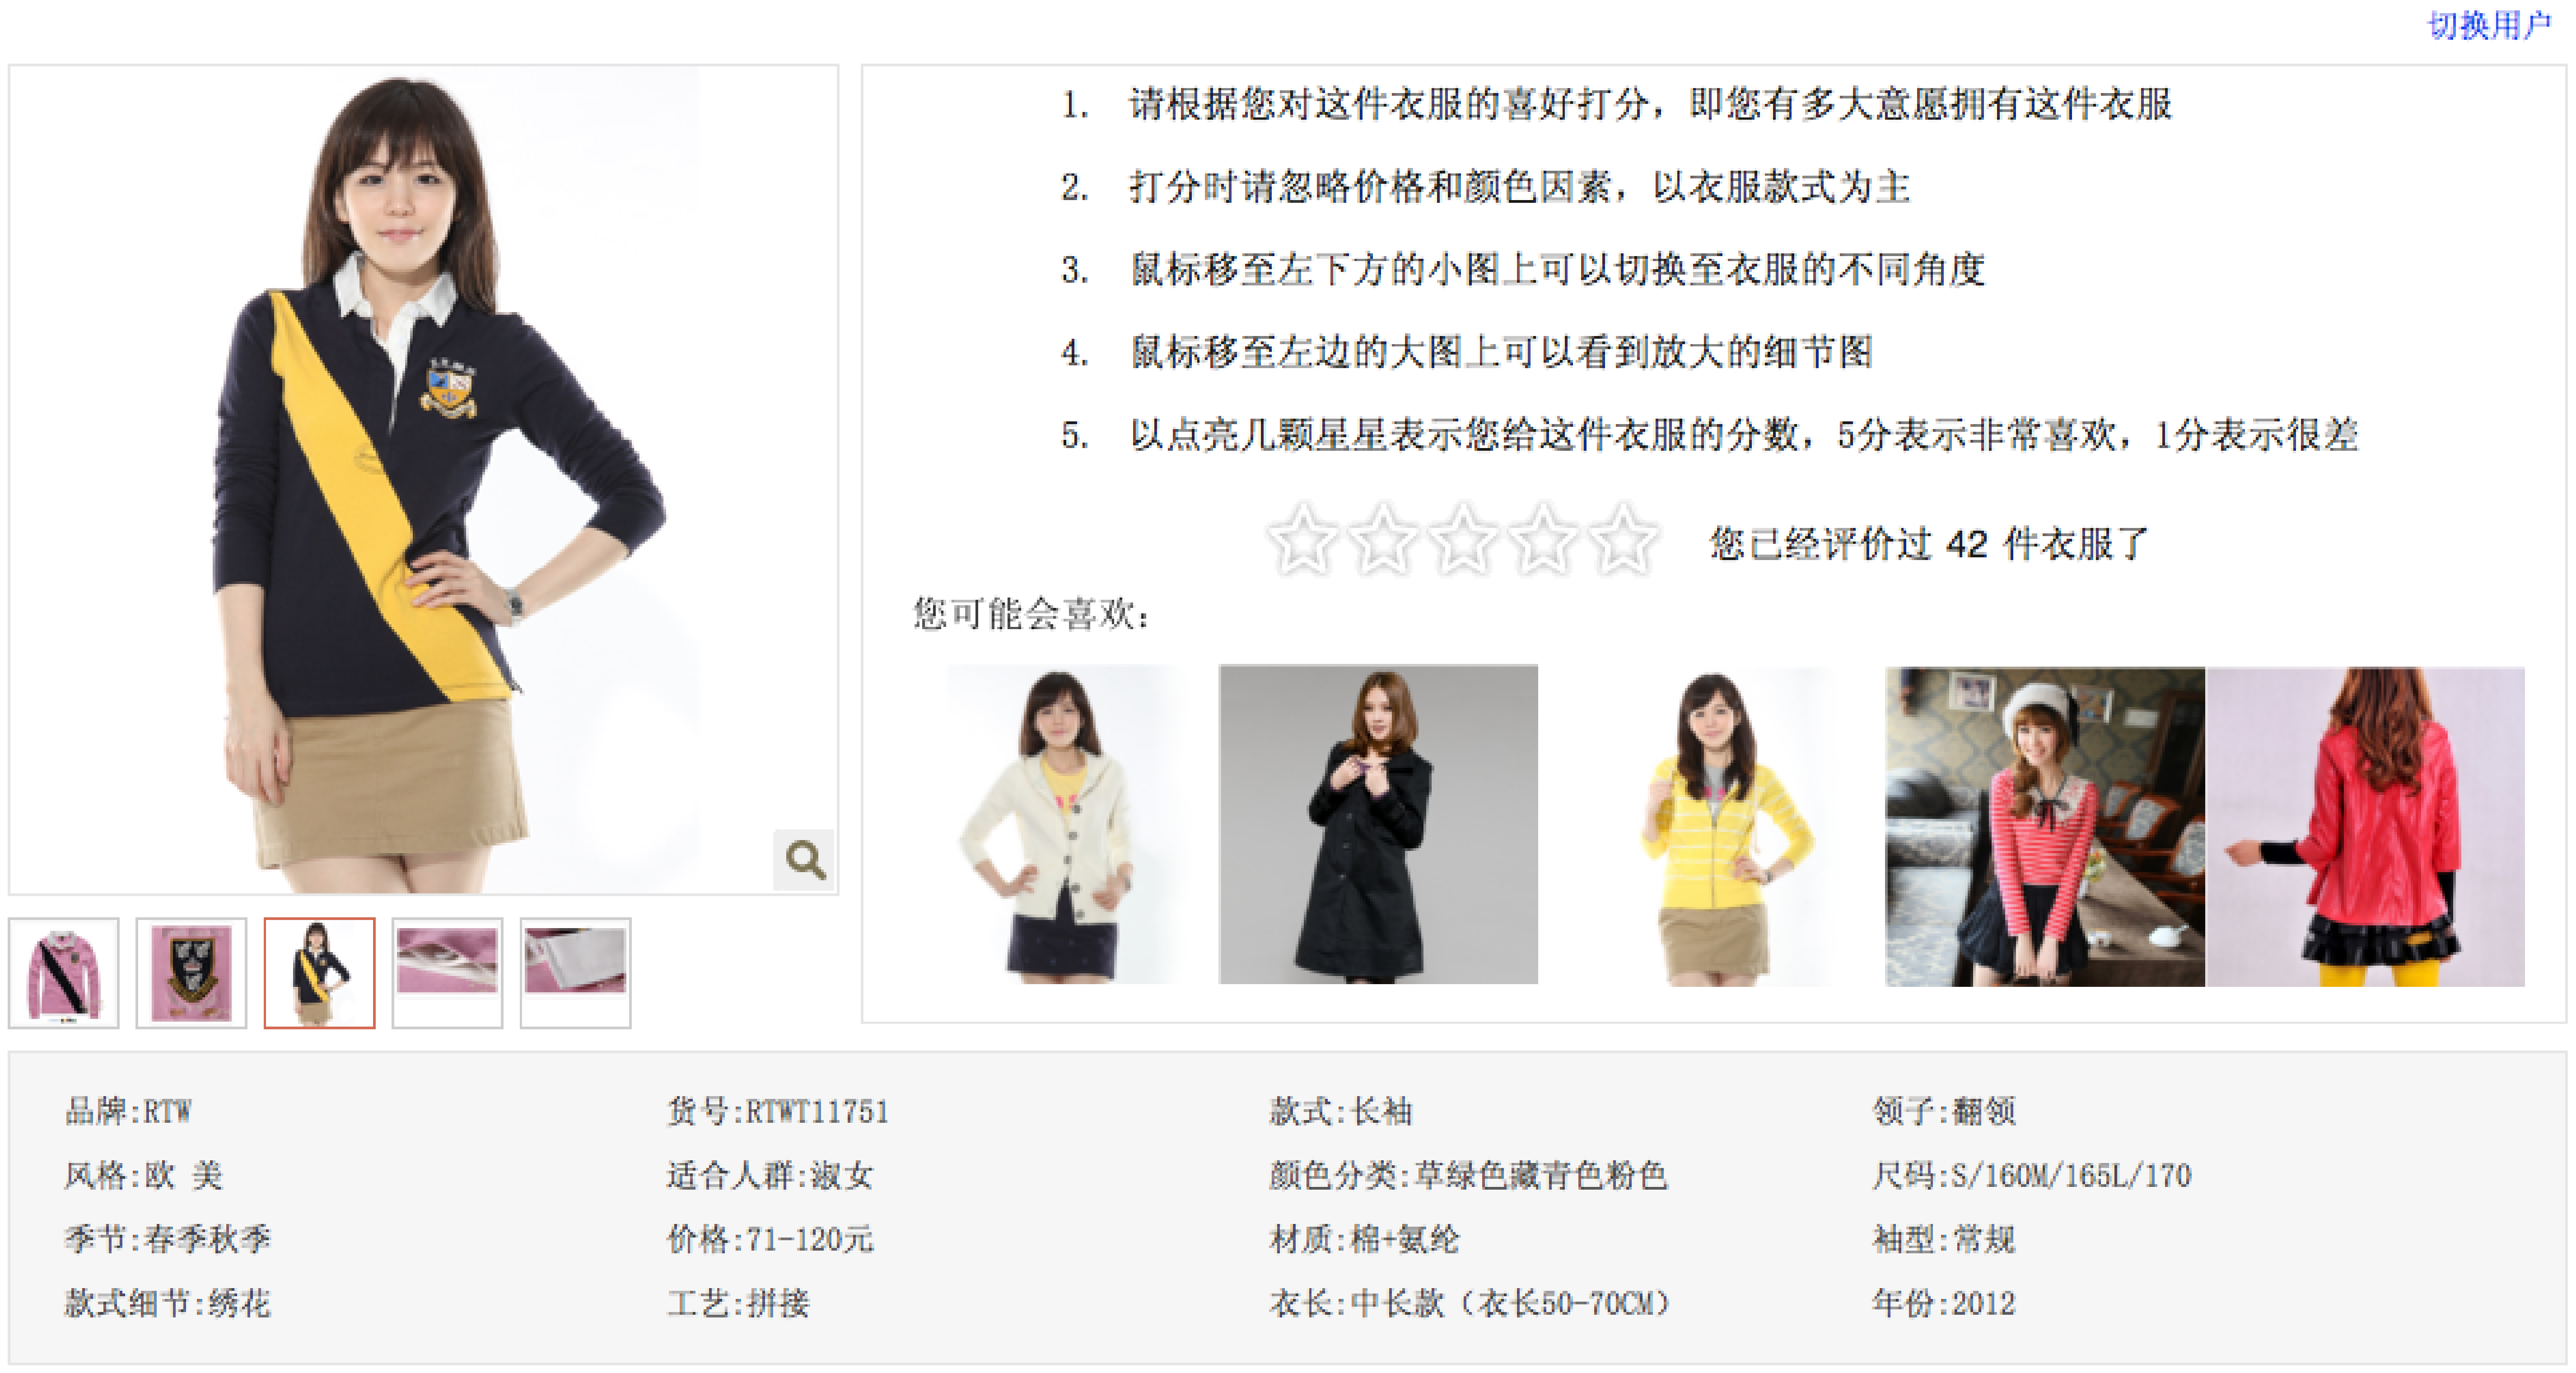
\includegraphics[width=0.8\textwidth]{website1}}
  \qquad
  \subfigure[Screenshot of viewing details of a product image]{
    \label{fig:website2}
    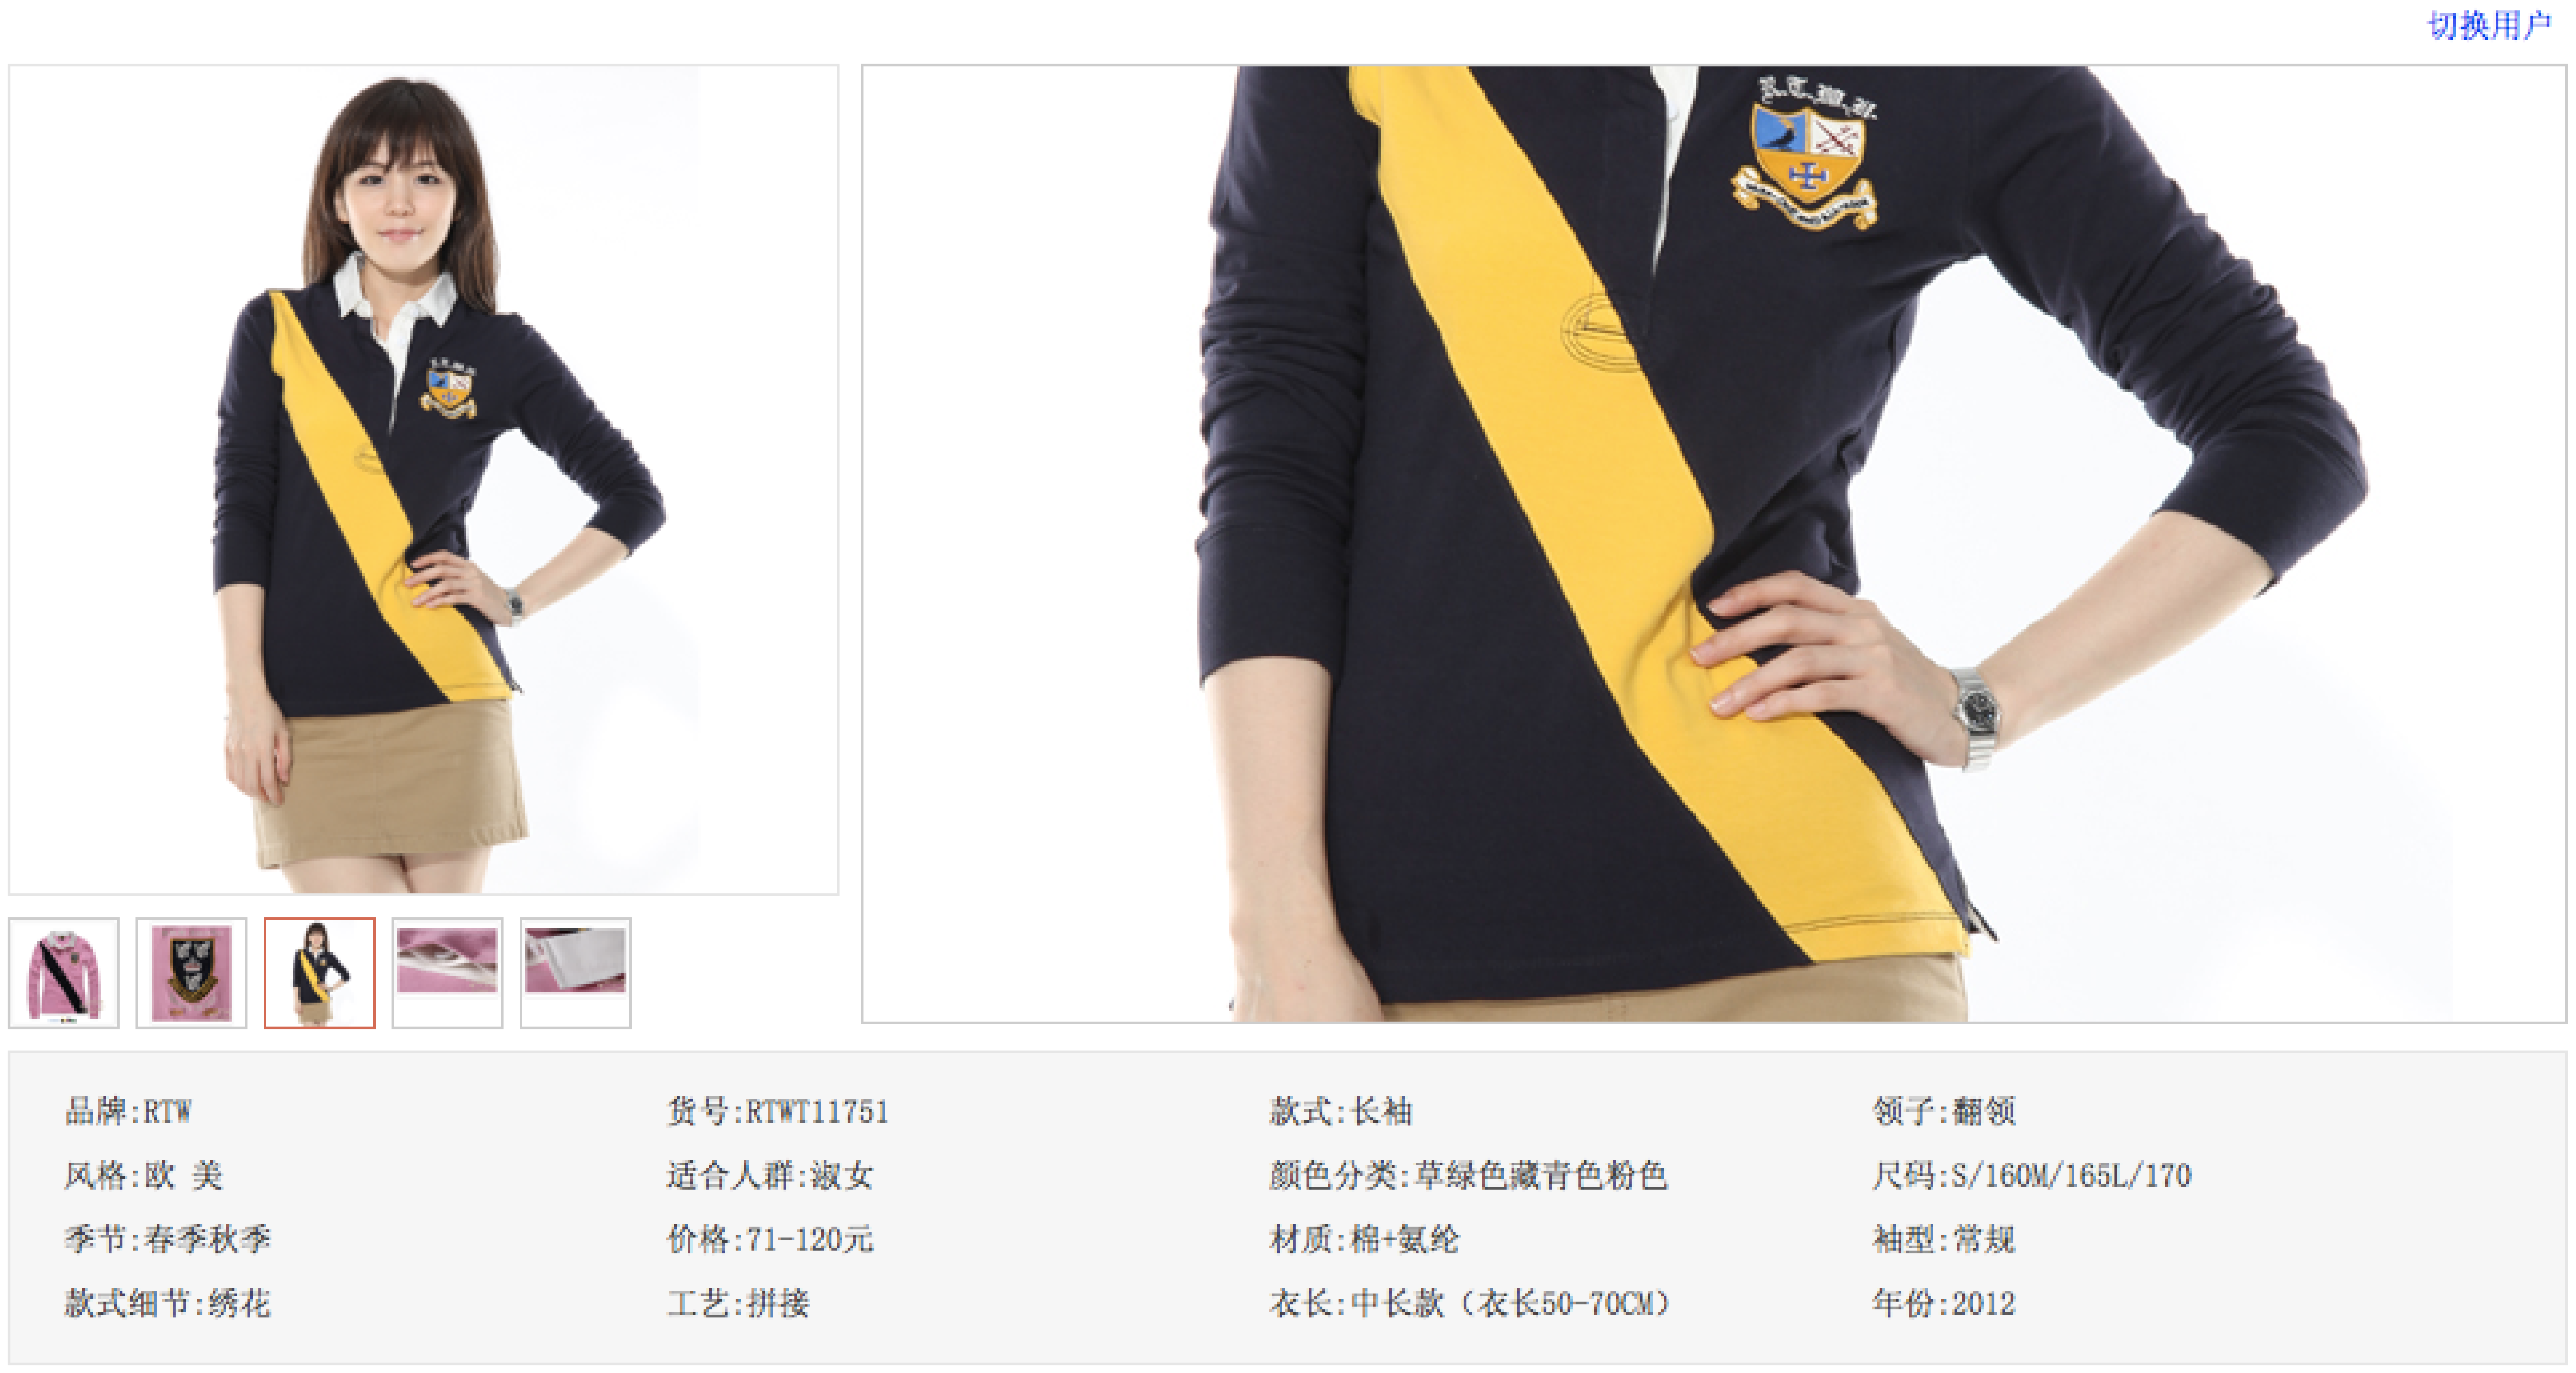
\includegraphics[width=0.8\textwidth]{website2}}
  \caption{Screenshots of our website for collecting user preferences}
  \label{fig:website}
\end{figure}

The website is written in PHP and deployed on Linux with Apache HTTP server. It randomly displays unrated products to the current user, collects user ratings of the products, and stores the ratings to a relational database for further investigation. The source code is available at \url{https://github.com/stfairy/recsys-website}.


\subsection{Results and Interpretation}
After acquiring the necessary data as input of the SVM, we began our training and assessing. Since we focused on every volunteer's individuality and personal preferences, we performed  the learning process to every one. 
Table 1 shows the results of LIBSVM learning after parameter modification, with the accuracy of 5-fold cross-validation.It implies that even with text features alone the accuracies could be high enough to make recommendations. However it is worth noticing that over-fitting is prone to occur since the learning set we use are extremely small. It is expected that after combining graphical features this potential problem could be alleviated. 

\begin{table}
  \centering  % used for centering table
  \begin{tabular}{c c | c c} % centered columns (2 columns)
    \hline                        %inserts double horizontal lines
    UserID & Accuracy & UserID & Accuracy \\ [0.9ex] % inserts table 
    %heading
    \hline                  % inserts single horizontal line
    1 & 89.0511\% & 13 & 94.1176\% \\
    2 & 92.5373\% & 14 & 89.3939\% \\
    3 & 80.9122\% & 15 & 93.7500\% \\
    4 & 88.4615\% & 16 & 96.6667\% \\
    5 & 91.3462\% & 17 & 93.3333\% \\
    6 & 90.0000\% & 18 & 94.5946\% \\
    7 & 86.8852\% & 19 & 85.7143\% \\
    8 & 89.4737\% & 20 & 89.4231\% \\
    9 & 97.0588\% & 21 & 88.3721\% \\
    10 & 78.3019\% & 22 & 89.7059\% \\
    11 & 82.0755\% & 23 & 90.4762\% \\
    12 & 85.0000\% & 24 & 95.1613\% \\[1ex]  
    \hline %inserts single line
  \end{tabular}
  \caption{LIBSVM 5-fold cross-validation accuracies} % title of Table
  \label{table:nonlin} % is used to refer this table in the text
\end{table}


\section{Conclusion and Future Work}\label{sec:conclusion}


\section{Related Work}\label{sec:related}

Collaborative Filtering (CF) \cite{Goldberg92} has become a very common technique 
  for providing personalized recommendations, suggesting items based on the similarity 
  between users' preferences.
Sarwar \etal\cite{Sarwar01} analyzed different item-based recommendation generation algorithms 
  and stated that item-based algorithms provide dramatically better performance than 
  user-based algorithms.

Zhang \etal\cite{Zhang10} proposed an integrated diffusion-based algorithm, which is very much 
  different from collaborative filtering, with the help of collaborative tagging 
  information, and experimental results demonstrated significant improvement in accuracy, 
  diversification and novelty of recommendations. 
However, it is not an online algorithm and cannot give real-time response to the user activities.

WebCF-DT \cite{Kim02} is a personalized recommendation procedure based on Web usage mining, 
  product taxonomy, association rule mining, and decision tree induction. 
It relies heavily on behavior patterns and lacks understanding of recommended materials. 
Also they don't have a comparison with collaborative filtering and rule-based approaches, 
  therefore the effectiveness is not convincing.

INTRIGUE \cite{Ardissono03} is a prototype tourist-information server that recommends 
  sightseeing destinations and itineraries by taking into account the preferences of 
  heterogeneous tourist groups instead of individuals.
INTRIGUE uses a na\"ive polynomial formula for generating scores of items and thus has less 
  intelligence than approaches supported by machine learning techniques.


\bibliographystyle{abbrv}
\bibliography{recsys}

\begin{appendices}
  \section*{Appendix}
  \section{Crawl}

\subsection{Selected shops}
\begin{enumerate}
\item http://store.taobao.com/shop/view\_shop-b22399989259942b7b66c99c175a5100.htm
\item http://store.taobao.com/?shop\_id=56634
\item http://store.taobao.com/?shop\_id=59495864
\item http://store.taobao.com/?shop\_id=33483998
\item http://store.taobao.com/?shop\_id=62997280
\item http://store.taobao.com/?shop\_id=62800620
\item http://liuzstyle-1.taobao.com/?spm=11020*pv.2-3JyCq.2-3rU2Br
\item http://fsnz.tmall.com/shop/viewShop.htm
\item http://justylenz.tmall.com/shop/viewShop.htm
\item http://cfa.tmall.com/shop/viewShop.htm
\item http://ousibo.tmall.com/shop/viewShop.htm
\item http://bitnicha.tmall.com/shop/viewShop.htm
\item http://huijiao.tmall.com/shop/viewShop.htm
\item http://eptisonfs.tmall.com/shop/viewShop.htm?prt=1326439183738\&prc=1
\item http://yingxiang.tmall.com/shop/viewShop.htm
\item http://zhennuo.tmall.com/shop/viewShop.htm
\item http://lanjue.tmall.com/shop/viewShop.htm
\item http://store.taobao.com/view\_shop.htm?user\_number\_id=734349353
\item http://dianliyou.tmall.com/shop/viewShop.htm
\item http://yixuanmeier.tmall.com/shop/viewShop.htm
\item http://oqueenz.tmall.com/shop/viewShop.htm
\item http://goefir.tmall.com/shop/viewShop.htm
\end{enumerate}

\subsection{URL matchers}
\begin{verbatim}
http://item\.tmall\.com/item\.htm\?(spm=[-_0-9a-zA-Z.]+&)?id=\d+
http://item\.taobao\.com/item\.htm\?(spm=[-_0-9a-zA-Z.]+&)?id=\d+
http://detail\.tmall\.com/item\.htm\?(spm=[-_0-9a-zA-Z.]+&)?id=\d+
\end{verbatim}

\subsection{\tt url.fetcher.sh}
\begin{verbatim}
#!/bin/bash

UA='Some User Agent'
item_counter=0

touch url.list
unlink url.list

for store in `cat stores.txt`; do
  echo "Fetch store information: $store"
  wget -q -U "$UA" -O - "$store" | cat > store.html.tmp
  for regex in `cat url.matchers`; do
    for url in `cat store.html.tmp | grep -o -P "$regex"`; do
      let item_counter=item_counter+1
      echo "    $item_counter: $url"
      echo $url >> url.list
    done
  done
  unlink store.html.tmp
done
cat url.list | wc -l

cat url.list | sort | uniq | cat > url.list.tmp
mv url.list.tmp url.list
cat url.list | wc -l
\end{verbatim}

\subsection{\tt item.fetcher.sh}
\begin{verbatim}
#!/bin/bash

UA='Some User Agent'
item_counter=0

touch id.list
unlink id.list

for url in `cat url.list`; do
  let item_counter=item_counter+1

  id=`echo $url | grep -o -P '(?<=id=)\d+'`
  echo $id >> id.list
  echo "Fetching item ($item_counter, id: $id): $url"

  item_dir="items/$id"
  rm -rf $item_dir
  mkdir $item_dir

  item_page="$item_dir/$id.html"
  wget -q -U "$UA" -O - "$url" > $item_page
  cat $item_page | wc -l
done
\end{verbatim}

\subsection{\tt image.fetcher.sh}
\begin{verbatim}
#!/bin/bash

UA='Some User Agent'
item_counter=0

for id in `cat id.list`; do
  item_page=`printf "items/%d/%d.html" $id $id`
  item_desc=`printf "items/%d/%d.txt" $id $id`
  top_jpg_dir=`printf "items/%d/top" $id`
  top_jpg_list=`printf "items/%d/top.txt" $id`

  let item_counter=item_counter+1
  echo "$item_counter: Fetching item $id..."

  cat $item_page
    | grep -P -A 1 '<ul class="attributes-list">'
    | grep -o -P '(?<=">).+?(?=</li>)'
    | sed 's/\&nbsp;//g' > $item_desc
  cat $item_page
    | grep -P -A 1 '<div class="tb-pic tb-s40">'
    | grep -o -P 'http://.+?\.jpg'
    | sort
    | uniq > $top_jpg_list

  rm -rf $top_jpg_dir
  mkdir $top_jpg_dir

  for jpg in `cat $top_jpg_list`; do
    wget -q -U "$UA" -P "$top_jpg_dir" "$jpg"
  done
done
\end{verbatim}

  \section{Classification}
\lstset{language=Matlab}
\begin{lstlisting}
function mvfile

disp('');
disp('**********Movefile**********');
disp('');

% File path
pathstr = fileparts(which('mvfile'));
dirname = fullfile(pathstr, 'recsys');
filelist = dir(dirname);
fid = fopen('result.txt');
cline = fgetl(fid);
while cline ~= -1
    [sourcefile, remain] = strtok(cline);
    [cluster, destfile] = strtok(remain);
    printf('Sourcefile:%s,destfile:%s\n',sourcefile,destfile);
    flag = exist(destfile, 'dir');
    if (flag == 0)
        mkdir(destfile);
    end
    printf('Move file %s to file %s\n',sourcefile,destfile);
    movefile(sourcefile, destfile);
    cline = fgetl(fid);
end

fclose(fid);
disp('**********MoveFileDone!**********');
\end{lstlisting}

\end{appendices}

\end{document}
